\begin{figure}[htb!]
\centering
\begin{tabular}{ccc}
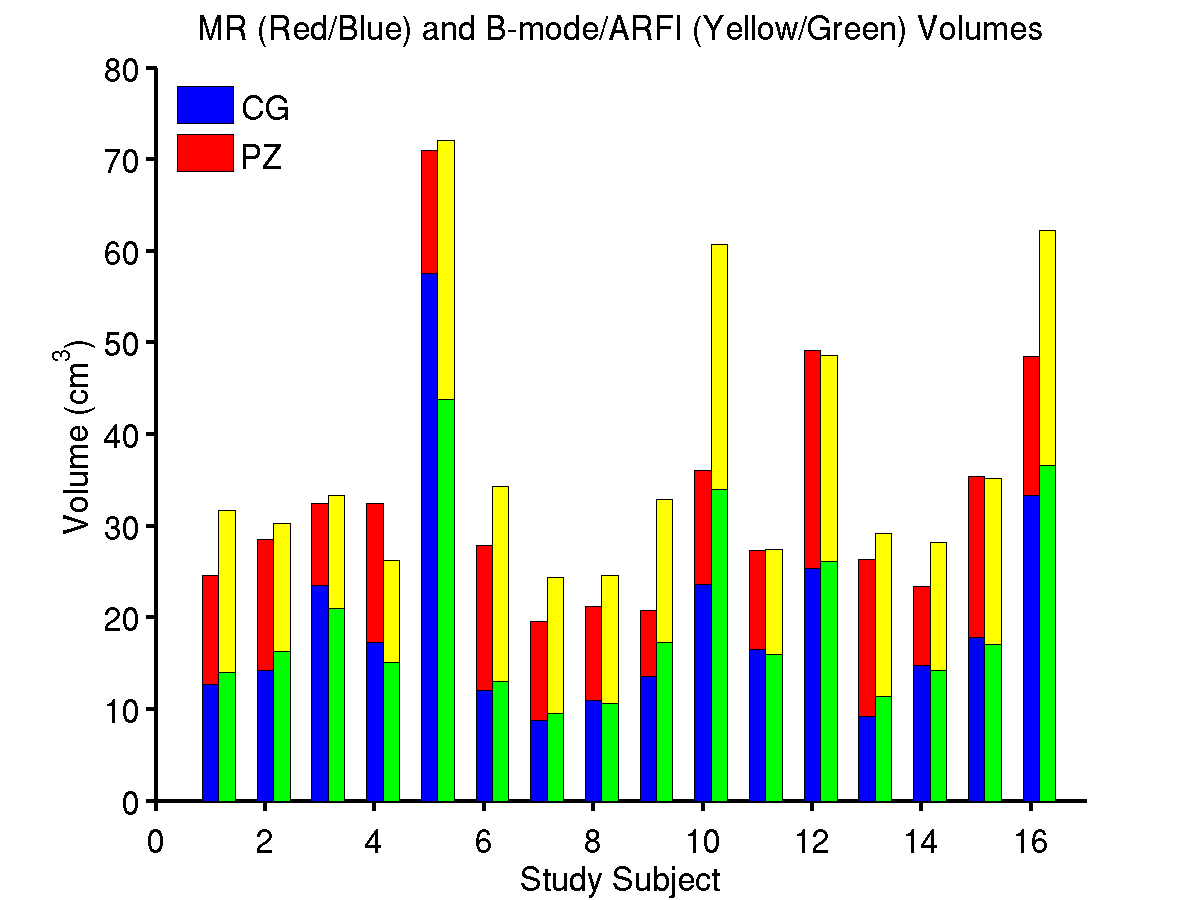
\includegraphics[width=0.3\linewidth]{figs/mr_arfi_volumes} &
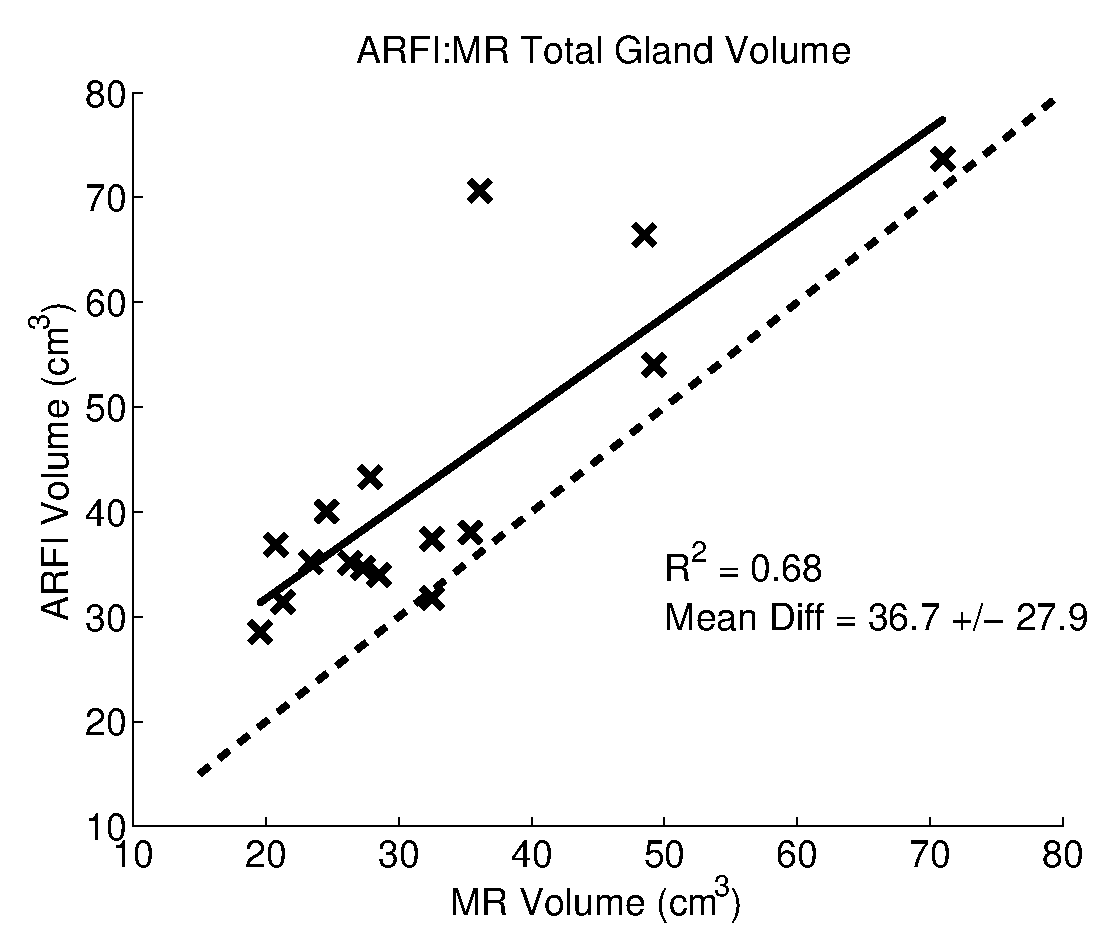
\includegraphics[width=0.3\linewidth]{figs/mr_arfi_total_linreg} &
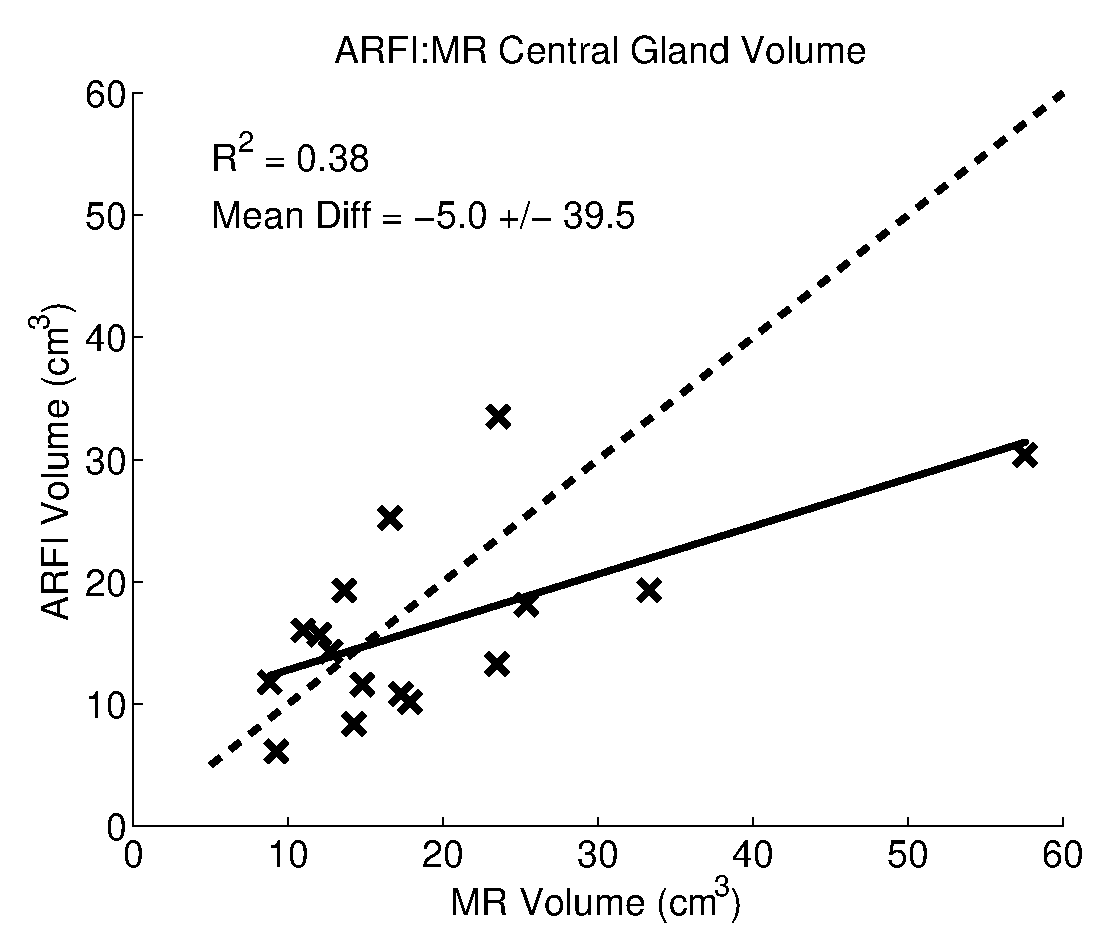
\includegraphics[width=0.3\linewidth]{figs/mr_arfi_central_linreg} \\
(a) CG:PZ Volume & (b) Total Gland Volume & (c) Central Gland Volume \\
\end{tabular}
\caption{Comparison of MR and ARFI zonal anatomy volume estimates from
    manually-segmented images.  Total prostate gland volumes ranged from
    19.6--71.0 cm$^3$ based on MR image models (a), with a moderate correlation
    between MR and ARFI imaging for both the total gland volume (R$^2$ =
    \MRarfiVolTotalRsq, (b)) and the central gland (R$^2$ =
    \MRarfiVolCentralRsq, (c)).  The ARFI total gland volumes had a positive
    bias compared with the MR volumes (\MRarfiVolTotalMeanDiff~$\pm$
    \MRarfiVolTotalStdDiff\% (b)), while the ARFI central zone volumes were on
    average more similar (\MRarfiVolCentralMeanDiff~$\pm$
    \MRarfiVolCentralStdDiff\%, (c)), but with some significant variability
    between study subjects.  Table~\ref{tab:mr_arfi_volumes} contains the
    individual volume estimates for the total prostate and central glands.}
\label{fig:mr_arfi_volumes} 
\end{figure}
